\section{Músicas e Efeitos Sonoros/Trilha Sonora}

\subsection{Introdução ao tema}
A trilha sonora é composta por todos os áudios presentes no aplicativo, tais como músicas (de menus ou de background), efeitos especiais, vozes e efeitos de personagens e narrações - quando houver necessidade.

A proposta da trilha sonora é criar ambiência, de modo a melhorar a imersão no jogo e garantir feedback mais eficiente e claro das ações tomadas pelo personagem (controlado pelo jogador), ações de inimigos, estímulos, obstáculos e NPCs
\footnote{Non-player character (Personagem não jogável) - compreende um personagem que não pode ser controlado pelo jogador, embora possa fazer parte da ação do jogo.}. 
A trilha sonora deve ainda valorizar o uso do software, de modo a permitir novas possibilidades de interação e comunicação com o usuário, indo além das informações visuais que não atenderiam ao uso do mesmo ou o tornaria seu uso menos interativo, mais lento e cansativo.

A narração é um componente da trilha sonora que deve ser produzido de forma cuidadosa, principalmente em jogos direcionados para público infantil ou em processo de alfabetização, pois guiará as ações do jogador e permitirá uma ação mais rápida e efetiva em caso de dúvidas ou orientações quanto ao jogo.

A produção da trilha sonora pode ocorrer de três maneiras:
\begin{itemize}
\item Captação do áudio da voz humana, de instrumentos musicais ou de objetos sonoros
\footnote{Compreendem objetos, que não são necessariamente instrumentos musicais, mas que emitem sons que podem ser aproveitados em criações artísticas e musicais. São elementos de criação estudados por diversos compositores, destacando-se Pierre Henri Marie Schaeffer.}, 
através de gravadores digitais ou computadores conectados com outros periféricos, como placa de som, microfones e mesas de som, utilizando-se de softwares específicos para isso: Sound Forge, Audacity, Sonar entre outros disponíveis no mercado. O resultado obtido normalmente é um arquivo de áudio.
\item Produção através de recursos MIDI
\footnote{Musical Instrument Digital Interface - compreende uma interface de comunicação entre dispositivos que se utilizem deste protocolo. Estes dispositivos podem ser computadores, instrumentos musicais e placas de som.}
, uma estrutura de dados, ou seja, não compreendendo áudios. Estes dados funcionam como uma ``partitura'' que o computador consegue entender através de softwares específicos, como o Sonar e o Reason. Obtém-se como resultado, arquivos de dados com a extensão ``mid''.
\item Os programas citados conseguem ``tocar'' esta ``partitura'' e gerar um arquivo de áudio, através da ligação pela interface MIDI, com bancos de sons instalados no computador, ou em instrumentos que se utilizem desta estrutura. Essas ``partituras'' podem ser criadas e editadas em programas de edição musical com o Sibelius, Finale, Encore e MuseScore.
\item Composições interativas e composições algorítmicas geradas por softwares específicos como o Pure Data ou o Max/MSP. Para este tipo de composição é possível utilizar linhas de programação, como por exemplo, a linguagem C, e também em tempo real. Neste caso, o áudio é gerado através de algoritmos inseridos e processados no computador.
\end{itemize}

É importante ressaltar que músicas prontas também podem ser utilizadas e alteradas, desde que as autorizações pertinentes sejam obtidas ou que não sejam protegidas por Leis de Direitos Autorais
\footnote{Artigo 41 da Lei nº 9.610/98: relata que os direitos autorais perduram por setenta anos, a partir de 1º de janeiro do ano subsequente ao falecimento do compositor. Muitos outros artigos compreendem leis que devem ser de conhecimento do produtor musical.}. 

Este trabalho de produção pode ser elaborado em um software multipista, como o Cakewalk Sonar, que permite manipular simultaneamente informação MIDI e áudio. Na captura de tela da Figura \ref{img:midi}, retirada de Jesus (2008), observa-se as trilhas ou tracks, nas cores rosa escuro (bateria), amarelo (baixo), azul (percussão) e ciano (hammond) que compreendem informações MIDI (sinalizada como), indicada pelos traços que representam a ``partitura'' para o computador. Já a trilha em cinza escuro (guitarra) é composta por um áudio (sinalizado por ) proveniente de captação em linha, ou seja, com o instrumento conectado em uma mesa ou placa de som ou da captação realizada através de microfone. 

\begin{figure}[!ht]
 \centering
 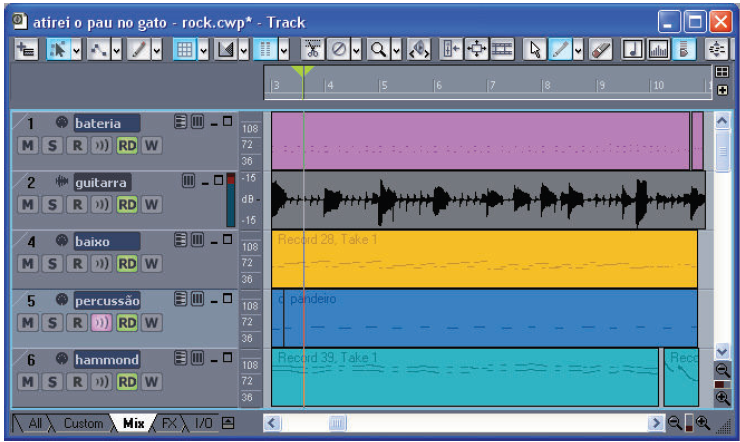
\includegraphics[scale=0.8]{musica_midi.png}
 \caption{Captura de tela demonstra as trilhas de áudio e MIDI. \cite{bib:musica_jesus}}
 \label{img:midi}
\end{figure}

A vantagem do uso de um software com estas características reside na rapidez da produção e na possibilidade de ouvir o resultado a ser obtido durante o processo, sem necessidade de finalizar o MIDI e o áudio em separado.
Outro software que apresenta como característica a produção musical estruturada em recursos MIDI e em áudio, é o Reason, da Empresa Propellerhead, que permite a conexão de instrumentos MIDI, gravando-os diretamente, ou importando arquivos ``.mid'' previamente elaborados em editores de partituras. Com o arquivo ``aberto'' dentro do Reason é possível alterá-lo ou acrescentar efeitos, como reverb
\footnote{Efeito que simula a reverberação do som em ambientes diversos.}
, chorus
\footnote{Efeito que simula a sensação de aumento das fontes sonoras.}
, flanger
\footnote{Efeito simular ao chorus, embora soando como se houvessem interferências no áudio.} 
e alterar o timbre
\footnote{Timbre corresponde à qualidade do som que nos permite identificar um instrumento, por exemplo, timbre do violão ou timbre da flauta.}
, ou seja, a qualidade do som a ser ouvida. Observa-se uma imagem do rack do Reason, com  uma ``prateleira'' e equipamentos virtuais, na Figura \ref{img:reason}.

\begin{figure}[!ht]
 \centering
 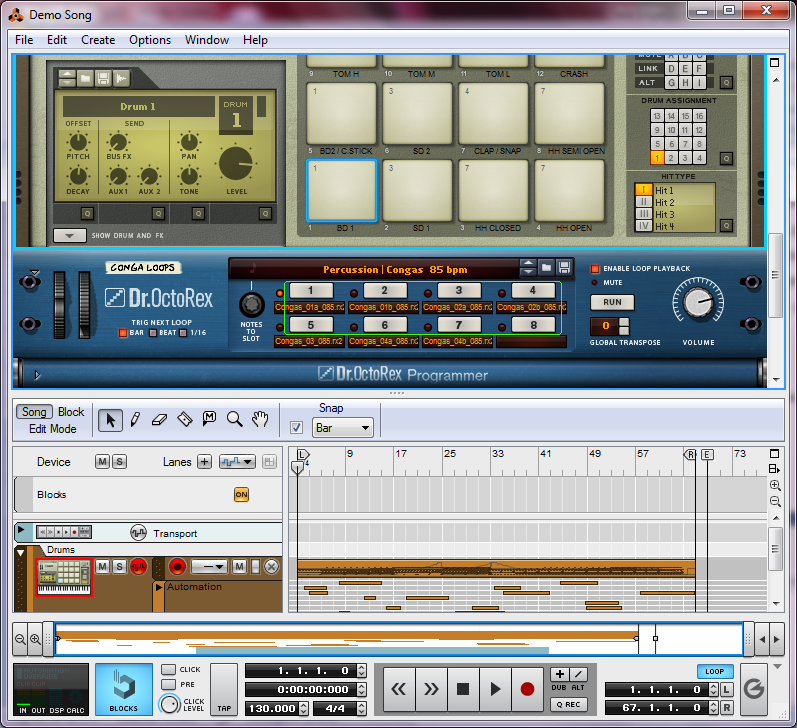
\includegraphics[scale=0.6]{musica_reason.png}
 \caption{Captura de tela do software Reason}
 \label{img:reason}
\end{figure}

Este software faz ainda o uso de refills ou banco de sons, permitindo a utilização de sons sampleados9 de alta fidelidade, tornando o som MIDI, desde que bem estruturado, praticamente equiparável ao de gravações de instrumentos reais. Samples ou amostras com resolução de 16 ou 24 bits são necessárias para se obter esta qualidade, bem como amostragem de 44.100 Hertz ou superior. 
A produção do áudio pode ser ainda incrementada utilizando-se recursos de um game engine como o Unity, que permite tornar efeitos sonoros mais realistas. Um exemplo possível ocorre quando o personagem se aproxima de uma fonte sonora, como o fogo, neste momento a intensidade sonora aumentará.

\subsection{Propostas de sonorização para o jogo ``As crônicas de Medrash''}

\subsubsection{Efeitos sonoros}
(descrever) cobra, urso, jacaré e tigre

\subsubsection{Áudios para menus}
\subsubsection{Músicas de background}